% Канонический TikZ-рисунок варианта 33. Править только здесь.
\newcommand{\figTangentSecant}{%
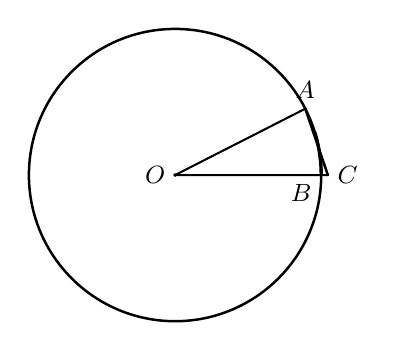
\begin{tikzpicture}[scale=0.58,line cap=round,line join=round,every node/.style={font=\small}]
  \def\R{3.2}\pgfmathsetmacro{\cx}{\R/cos(17)}
  \coordinate (O) at (0,0); \coordinate (B) at (0:\R);
  \coordinate (A) at (27:\R); \coordinate (C) at (\cx,0);
  \draw[line width=0.9pt] (O) circle (\R); \draw[line width=0.9pt] (A)--(C);
  \draw[line width=0.75pt] (O)--(A) (O)--(C);
  \draw[line width=1.2pt] (B) arc (0:17:\R);
  \fill (O) circle (1.2pt); \node[left] at (O) {\(O\)};
  \node[above] at (A) {\(A\)}; \node[below left] at (B) {\(B\)};
  \node[right] at (C) {\(C\)};
\end{tikzpicture}
}
